\section{动量守恒}\label{sec:08.01}

迄今为止,我们大都讨论单个质点的运动。在这一章里,我
们要讨论由许多质点构成的体系的运动规律。这种问题,常称为
质点系问题,或多体问题。例如,由所有行星和太阳构成的太阳
系就是一个典型的质点系。一般在质点系中,每个质点都要受到
其他质点的作用,同时,也受到体系之外的物体的作用。地球不
但要受到太阳的万有引力作用,而且与其他所有行星都有万有引
力作用。显然,在质点系中,每个质点的运动一般是相当复杂
的。

在质点系中有一类是特别的,即所有质点都没有受到体系之
外的物体的作用力。也可以简单地说,整个体系不与外物相互作
用,这种质点体系称为孤立体系。在现实世界中,当然没有严格
的孤立体系,但是近似的孤立体系很多。所谓近似的,是指体系
内部的相互作用远大于外物对体系的作用,即每个质点所受内力
远大于它所受的外力。譬如太阳系,除了太阳与行星、行星与行
星之间的引力之外,当然也受到其他恒星的作用,但是这种力比
较小,所以太阳系就是一个近似的孤立体系。又如一个大分子,
它是由许多原子组成,原子之间的相互作用远大于其他分子的作
用,这样,我们也可以把这个大分子看作近似的孤立体系。再如,
% 227.jpg
在加速器的实验中,高能粒子束打到靶上,发生各种反应,我们
\clearpage\noindent
称之为碰撞。看起来这个系统非常复杂,但由于碰撞时作用很强,
我们可以把一个高能粒子与它所撞上的一个粒子作为孤立体系来
处理,其他作用全可不顾及。

\begin{wrapfigure}[5]{r}{13em}
  \vspace{-1.5em}
  \centering
  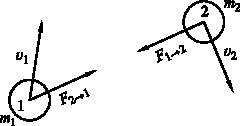
\includegraphics{figure/fig08.01}
  \caption{二质点体系}
  \label{fig:08.01}
\end{wrapfigure}
孤立体系有些共同的动力学规律,其中之一就是总动量守恒。

我们首先讨论一个最简单的质点系,它只包括两个质点1及
2(图81)。如果它是孤立体系,那么,作用在质点1上的力,只
有2对它的作用力$ \vec { F } _ { 2 \to 1 } $而作用在质点2上的力,只有1对它的
作用力$ \vec { F } _ { 1 \to 2 } $。故根据牛顿第二定律,有
\begin{equation}\label{eqn:08.01.01}
  \begin{split}
    m _ { 1 } \frac { \dif \vec { v } _ { 1 } } { \dif t } = \vec { F } _ { 2 \to 1 }  \\
    m _ { 2 } \frac { \dif \vec { v } _ { 2 } } { \dif t } = \vec { F } _ { 1 \to 2 }
  \end{split}
\end{equation}
上述两方程就是体系的动力学基本方程。再根据牛顿第三定律
\begin{equation*}
  \vec { F } _ { 1 \to 2 } = - \vec { F } _ { 2 \to 1 }
\end{equation*}
即可由式(\eqref{eqn:08.01.01})推得
\begin{equation*}
  m _ { 1 } \frac { \dif \vec { v } _ { 1 } } { \dif t } + m _ { 2 } \frac { \dif \vec { v } _ { 2 } } { \dif t } = 0
\end{equation*}
它可改写为
\begin{equation}\label{eqn:08.01.02}
  \frac { \dif } { \dif t } \left( m _ { 1 } \vec { v } _ { 1 } + m _ { 2 } \vec { v } _ { 2 } \right) = 0
\end{equation}
我们定义
\begin{equation}\label{eqn:08.01.03}
  \vec{ P } \equiv m _ { 1 } \vec { v } _ { 1 } + m _ { 2 } \vec { v } _ { 2 }
\end{equation}
所以,式\eqref{eqn:08.01.02}成为
\begin{equation}\label{eqn:08.01.04}
  \frac { \dif \vec { P } } { \dif t } = 0
\end{equation}
% 228.jpg
最终得到\vspace{-1.56em}
\begin{equation}\label{eqn:08.01.05}
  \vec { P } = \text { 不变量 }
\end{equation}
此式表明,对于两个质点构成的孤立体系,我们找到了一个新的
不变量$ \vec { P } $,称它为动量。在证明过程中,我们并没有用到作用力
的具体形式,只用了牛顿第二、三定律,所以,这个守恒律是非
常普遍的,即与作用力的具体形式无关,无论力是保守的或非保
守的都适用。

对于多个质点所构成的孤立体系,可以用完全类似的方法证
明体系的总动量不随时间变化,即
\begin{equation}\label{eqn:08.01.06}
  \begin{aligned}
    P & = m _ { 1 } \vec { v } _ { 1 } + m _ { 2 } \vec { v } _ { 2 } + \cdots + m _ { n } \vec { v } _ { n } \\
      & = \text { 不变量 }
  \end{aligned}
\end{equation}
或者\vspace{-1.56em}
\begin{equation}\label{eqn:08.01.07}
  \frac { \dif \vec { P } } { \dif t } = 0
\end{equation}
这就是动量守恒定律。

对于单个质点,我们也可以定义它的动量为$ \vec { P } = m \vec { v } $ ,那么,
动量守恒\lhbrak 式\eqref{eqn:08.01.06}\rhbrak 可以表述为
\begin{equation}\label{eqn:08.01.08}
  \vec { P } = \sum _ { i = 1 } ^ { n } \vec { P } _ { i } = \text { 不变量 }
\end{equation}
其中$ \vec { P } _ { i } $是第$ i $个质点的动量。上式表示,在孤立体系中,每个质点
的动量时刻在变化着,但它们的总和不变。

当体系与外界有相互作用,即非孤立状态时,动量守恒一般
不成立,但当外力总合为零时,式\eqref{eqn:08.01.08}仍然成立。

迄今我们已经研究过两条守恒定律了,即能量守恒定律与动
量守恒定律。下面我们比较一下这两条守恒定律的特点。

(1)动量是矢量,动量守恒\lhbrak 式\eqref{eqn:08.01.08}\rhbrak 是一个矢量关系式,
即实际上包括三个不变量:
\begin{equation*}
  \begin{aligned}
    P _ { x } = \text { 不变量 } \\
    P _ { y } = \text { 不变量 }
  \end{aligned}
\end{equation*}
% 229.jpg
\begin{equation}\label{eqn:08.01.09}
  P _ { z } = \text { 不变量 }
\end{equation}
而能量是标量,能量守恒只给出一个不变量。

(2)动量守恒定律与机械能守恒定律是相互独立的。因此,对
一个具体的物理过程而言,机械能守恒定律的成立,并不决定动
量守恒定律成立反过来,动量守恒定律的成立,也不决定机械
能守恒定律成立。譬如,我们可以找到许多能量守恒成立而动量
守恒不成立的例子。对于行星沿圆轨道绕太阳的运动,若把行星
作为一个体系,它的能量是守恒的,但是动量并不守恒,因为速
度方向时刻变化着。反过来,动量守恒成立而机械能守恒不成立
的例子也很多如果体系中的质点之间有摩擦力存在,则机械能
守恒定律不成立,但动量守恒定律是成立的。这些例子都表明,
两条守恒定律是不能互相代替的。能量、动量与位置、速度、质
量、加速度等一样,是有不可替代作用的动力学量。

(3)在证明动量守恒定律时,我们用到了牛顿第三定律。第三
章中我们已经指出,牛顿第三定律是关于力的性质的一个定律;
并且也已指明,第三定律并非总是适用的。因此,只有在第三定
律适用的地方,才可以应用动量守恒定律。反之,我们也能从动
量守恒的成立,证明第三定律的正确,它们互为因果。在经典力
学中,它们二者是等价的。

总之,在经典力学中,机械能守恒适用于保守力的情况,而
动量守恒适用于牛顿第三定律成立的情况。

\example 一炮弹以速度$ \vec { F } $飞行,突然分裂为两个质量相等的碎
片向两旁飞去。已知其中一块碎片的速度大小仍为$ v $,但方向与原
炮弹方向成$ 60 ^ { \circ } $角。试求另一碎片的速度$ \vec { v } _ { 2 } $,分裂前后的机械能守
恒吗?

\resolve 炮弹在炸裂的瞬间,由于炸药的化学能转变为炮弹的机
械能,而且在这一瞬间内力的作用远大于外力(例如重力)的作用,
故可以近似看成孤立系统,即炮弹分裂的前后,系统的动量保持
% 230.jpg
不变。在图\ref{fig:08.02}所示的坐标系中,在$ x $方向
% TODO: \usepackage{graphicx} required
\begin{figurex}
  \centering
  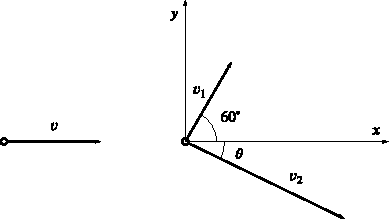
\includegraphics{figure/fig08.02}
  \caption{}
  \label{fig:08.02}
\end{figurex}
\begin{equation*}
  \begin{split}
    m v &= \frac { m } { 2 } \left( v _ { 1 } \cos 60 ^ { \circ } + v _ { 2 } \cos \theta \right)  \\
    &= \frac { m } { 2 } \left( v \cos 60 ^ { \circ } + v _ { 2 } \cos \theta \right)
  \end{split}
\end{equation*}
在$ y $方向
\begin{equation*}
  \begin{split}
    0 &= \frac { m } { 2 } \left( v _ { 1 } \sin 60 ^ { \circ } - v _ { 2 } \sin \theta \right)  \\
    &= \frac { m } { 2 } \left( v \sin 60 ^ { \circ } - v _ { 2 } \sin \theta \right)
  \end{split}
\end{equation*}
由上两式可得
\begin{equation*}
  \begin{split}
    v \left( 2 - \cos 60 ^ { \circ } \right) &= v _ { 2 } \cos \theta  \\
    v \sin 60 ^ { \circ } &= v _ { 2 } \sin \theta
  \end{split}
\end{equation*}
因此可以求得
\begin{equation*}
  \tg \theta = \frac { \sin 60 ^ { \circ } } { 2 - \cos 60 ^ { \circ } } = \frac { 1 } { \sqrt { 3 } }
\end{equation*}
即\vspace{-1.56em}
\begin{equation*}
  \theta = 30 ^ { \circ }
\end{equation*}
又\vspace{-1.56em}
\begin{equation*}
  \begin{split}
    v _ { 2 } &= \frac { \sin 60 ^ { \circ } } { \sin 3 0 ^ { \circ } } v \\
    &= \sqrt { 3 } v = 1.73 v
  \end{split}
\end{equation*}
%\clearpage
%\vspace{-1.56em}
%\begin{equation*}
%	    % 231.jpg
%= \sqrt { 3 } v = 1.73 v
%\end{equation*}
故分裂前后动能之差为
\begin{equation*}
  \begin{split}
    \Delta T &= \left( \frac { 1 } { 2 } + m _ { 1 } v _ { 1 } ^ { 2 } + \frac { 1 } { 2 } m _ { 2 } v ^ { 2 } \right) - \frac { 1 } { 2 } m v ^ { 2 }  \\
    &= \frac { m } { 4 } \left( v ^ { 2 } + 3 v ^ { 2 } \right) - \frac { 1 } { 2 } m v ^ { 2 }  \\
    &= \frac { 1 } { 2 } m v ^ { 2 }
  \end{split}
\end{equation*}
动能增加了$ 1 $倍。这能量来源于化学能。

\example 在测量子弹速度时,往往用冲击摆。将质量为$ m _ 1 $的
重物(装砂的木箱)用$ 8 $根绳挂起,使它只能摆动,不能转动,绳
\begin{wrapfigure}[7]{r}{12em}
  \centering
  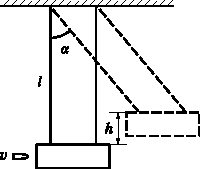
\includegraphics{figure/fig08.03}
  \caption{}
  \label{fig:08.03}
\end{wrapfigure}
长$ 1 $厘米(\ref{fig:08.03})。开始时重物静止,
将质量为$ m _ 2 $的子弹沿重物能够摆动
的方向水平地射入重物,$ m _ 1 $与$ m _ 2 $发生
完全非弹性碰撞,即碰后重物和子弹一起运动,而偏离其平衡位置最大到$ \alpha $
角。计算子弹在进入重物时的速度$ v $。

\resolve 子弹与$ m _ { 1 } $相碰时,在水平

方向没有外力作用,故以地球为参考系,以$ m _ 1 $,$ m _ 2 $为系统,在
水平方向系统的动量守恒。此后,子弹与$ m _ 1 $一起以速度$ u $运
动。由于$ \left( m _ { 1 } + m _ { 2 } \right) $上有重力$ \left( m _ { 1 } + m _ { 2 } \right) g $ 和张力$ T $作用,而张力始
终与位移方向垂直,不作功,故$ \left( m _ { 1 } + m _ { 2 } \right) $系统的机械能守恒
应用这两个守恒定律,可列出方程
\begin{equation*}
  \begin{split}
    &m _ { 2 } v = \left( m _ { 1 } + m _ { 2 } \right) u  \\
    &\frac { 1 } { 2 } \left( m _ { 1 } + m _ { 2 } \right) u ^ { 2 } = \left( m _ { 1 } + m _ { 2 } \right) g h
  \end{split}
\end{equation*}
解得\vspace{-1.56em}
\begin{equation*}
  \begin{split}
    &u = \sqrt { 2 g h }  \\
    &v = \left( \frac { m _ { 1 } + m _ { 2 } } { m _ { 2 } } \right) \sqrt { 2 g h }
  \end{split}
\end{equation*}
% 232.jpg
由几何关系知
\begin{equation*}
  \begin{split}
    h &= l \left( 1 - \cos \alpha \right) \\
    &= 2 l \sin ^ { 2 } \frac { \alpha } { 2 }
  \end{split}
\end{equation*}
所以得
\begin{equation*}
  v = \frac { 2 \left( m _ { 1 } + m _ { 2 } \right) } { m _ { 2 } } \sqrt { g l } \sin \frac { \alpha } { 2 }
\end{equation*}
其中$ m _ 1 $,$ m _ 2 $,$ g $,$ l $都是已知数,通过测量$ \alpha $可算出$ v $。